\documentclass[12pt,a4paper]{report}

%% Verze pro jednostranný tisk:
% Okraje: levý 40mm, pravý 25mm, horní a dolní 25mm
% (ale pozor, LaTeX si sám přidává 1in)
\setlength\textwidth{145mm}
\setlength\textheight{247mm}
\setlength\oddsidemargin{15mm}
\setlength\evensidemargin{15mm}
\setlength\topmargin{0mm}
\setlength\headsep{0mm}
\setlength\headheight{0mm}

% \openright zařídí, aby následující text začínal na pravé straně knihy
\let\openright=\clearpage

%% Použité kódování znaků
\usepackage[utf8]{inputenc}

%% Ostatní balíčky
\usepackage{graphicx}
\usepackage{amsmath}
\usepackage{amssymb}
\usepackage{latexsym}
\usepackage{mathtools}
%\usepackage{amsfonts}
\usepackage[noend]{algpseudocode}
\usepackage{algorithm}
\usepackage{url}
\usepackage{afterpage}
\usepackage{natbib}
\usepackage{verbatim}
\usepackage{rotating}
\usepackage{multirow}
%\usepackage{multicol}
\usepackage{tocbibind}
\usepackage[usenames,dvipsnames]{color}
\usepackage{subfig}

%% Balíček hyperref, kterým jdou vyrábět klikací odkazy v PDF,
%% ale hlavně ho používáme k uložení metadat do PDF (včetně obsahu).
\usepackage[hidelinks]{hyperref}
\hypersetup{pdftitle=Measures of Machine Translation Quality}
\hypersetup{pdfauthor=Matouš Macháček}

% Tato makra přesvědčují mírně ošklivým trikem LaTeX, aby hlavičky kapitol
% sázel příčetněji a nevynechával nad nimi spoustu místa. Směle ignorujte.
%\makeatletter
%\def\@makechapterhead#1{
%  {\parindent \z@ \raggedright \normalfont
%   \Huge\bfseries \thechapter. #1
%   \par\nobreak
%   \vskip 20\p@
%}}
%\def\@makeschapterhead#1{
%  {\parindent \z@ \raggedright \normalfont
%   \Huge\bfseries #1
%   \par\nobreak
%   \vskip 20\p@
%}}
%\makeatother

\def\parcite#1{\citep{#1}}
\def\perscite#1{\cite{#1}}

% Deklarace stylů fontů pro různé druhy termínů
\newcommand{\metric}[1]{\textsc{#1}}
\newcommand{\system}[1]{\textsc{#1}}
\newcommand{\pojem}[1]{\texttt{#1}}
\newcommand{\metoda}[1]{\textbf{#1}}
\newcommand{\script}[1]{\texttt{#1}}
\newcommand{\XXX}[1]{\textcolor{Red}{XXX #1}}
%\newcommand{\XXX}[1]{}
\newcommand{\best}[1]{\textbf{#1}}
\def\oosmark#1{\llap{$\wr$\,}#1}  % out-of-sequence mark
\newcommand*\Let[2]{\State #1 $\gets$ #2}
\newcommand{\hit}[1]{\textcolor{OliveGreen}{\textbf{#1}}}
\newcommand{\miss}[1]{\textcolor{Red}{\textbf{#1}}}
\newcommand{\worse}[1]{\textcolor{Red}{\textbf{W}}}
\newcommand{\better}[1]{\textcolor{OliveGreen}{\textbf{B}}}
\newcommand{\equal}[1]{\textcolor{Blue}{\textbf{E}}}
\newcommand{\vect}[1]{\boldsymbol{#1}}

\DeclareMathOperator{\cnt}{count}
\DeclareMathOperator{\len}{len}
\DeclareMathOperator*{\argmax}{arg\,max}
\DeclareMathOperator*{\argmin}{arg\,min}


\begin{document}

% Trochu volnější nastavení dělení slov, než je default.
\lefthyphenmin=2
\righthyphenmin=2

%%% Titulní strana práce

\pagestyle{empty}
\begin{center}

\large

Charles University in Prague

\medskip

Faculty of Mathematics and Physics

\vfill

{\bf\Large MASTER THESIS}

\vfill

\centerline{\mbox{\includegraphics[width=60mm]{img/logo}}}

\vfill
\vspace{5mm}

{\LARGE Matouš Macháček}

\vspace{15mm}

% Název práce přesně podle zadání
{\LARGE\bfseries Measures of \\ Machine Translation Quality}

\vfill

% Název katedry nebo ústavu, kde byla práce oficiálně zadána
% (dle Organizační struktury MFF UK)
Institute of Formal and Applied Linguistics

\vfill

\begin{tabular}{rl}

Supervisor of the master thesis: & RNDr. Ondřej Bojar, Ph.D. \\
\noalign{\vspace{2mm}}
Study programme: & Computer Science \\
\noalign{\vspace{2mm}}
Specialization: & Mathematical Linguistics \\
\end{tabular}

\vfill

% Zde doplňte rok
Prague 2014

\end{center}

\newpage

%%% Následuje vevázaný list -- kopie podepsaného "Zadání diplomové práce".
%%% Toto zadání NENÍ součástí elektronické verze práce, nescanovat.

%%% Na tomto místě mohou být napsána případná poděkování (vedoucímu práce,
%%% konzultantovi, tomu, kdo zapůjčil software, literaturu apod.)

\openright

I would like to thank my supervisor, RNDr. Ondřej Bojar, Ph.D., for his advice
and guidance. He taught me a lot over the years of my study and I am very
grateful to him for that. 

Many thanks go to annotators of machine translation quality. Without them,
there would be no manual evaluation experiment in my thesis.

I would like to also thank Markéta Šteflová for proofreading my thesis.

Finally, I would like to give special thanks to my girlfriend Bára for her
love, support, encouragement and patience throughout the countless hours I have
spent on this thesis. I would like to dedicate this thesis to her. 

\newpage

%%% Strana s čestným prohlášením k diplomové práci

\vglue 0pt plus 1fill

\noindent
I declare that I carried out this master thesis independently, and only with the cited
sources, literature and other professional sources.

\medskip\noindent
I understand that my work relates to the rights and obligations under the Act No.
121/2000 Coll., the Copyright Act, as amended, in particular the fact that the Charles
University in Prague has the right to conclude a license agreement on the use of this
work as a school work pursuant to Section 60 paragraph 1 of the Copyright Act.

\vspace{10mm}

\hbox{\hbox to 0.5\hsize{%
In Prague, 31th of July 2014 
\hss}\hbox to 0.5\hsize{%
%signature of the author
\hss}}

\vspace{20mm}
\newpage

%%% Povinná informační strana diplomové práce

\vbox to 0.5\vsize{
\setlength\parindent{0mm}
\setlength\parskip{5mm}

Název práce:
Měření kvality strojového překladu

Autor:
Matouš Macháček

Ústav:
Ústav formální a aplikované lingvistiky

Vedoucí diplomové práce:
RNDr. Ondřej Bojar, Ph.D., UFAL

Abstrakt: V této práci zkoumáme manuální i automatické metody pro vyhodnocování
kvality strojového překladu. Navrhujeme manální metodu evaluace, ve které
anotátoři hodnotí místo celých vět pouze krátké úseky strojového překladu, což
zjednodušuje a zefektivňuje anotaci. Provedli jsme anotační experiment a
vyhodnotili jsme systémy strojového překladu podle této metody. Získané
výsledky jsou velmi podobné těm z oficiálního vyhodnocení systémů v rámci
sotěže WMT14. Získanou databázi anotací dále používáme k evaluaci nových,
neviděných systému a k ladění parametrů statistického strojového překladače.
Evaluace nových systémů ale dává nepřesné výsledky a v práci proto analyzujeme
důvody tohoto neúspěchu. V rámci zkoumání automatických metod evaluace jsme
dvakrát po sobě organizovali soutěž strojových metrik v rámci workshopu WMT.  V
této práci uvádíme výsledky z poslední soutže, diskutujeme různé metody
metaevaluace a analyzujeme některé zúčastněné metriky. 

Klíčová slova:
strojový překlad, vyhodnocování kvality, automatické metriky, anotace


\vss} %\nobreak

\newpage

\vbox to 0.5\vsize{
\setlength\parindent{0mm}
\setlength\parskip{5mm}

Title:
Measures of Machine Translation Quality

Author:
Matouš Macháček

Department:
Institute of Formal and Applied Linguistics

Supervisor:
RNDr. Ondřej Bojar, Ph.D.

Abstract: We explore both manual and automatic methods of machine translation
evaluation. We propose a manual evaluation method in which annotators rank only
translations of short segments instead of whole sentences. This results in
easier and more efficient annotation. We have conducted an annotation
experiment and evaluated a set of MT systems using this method. The obtained
results are very close to the official WMT14 evaluation results. We also use
the collected database of annotations to automatically evaluate new, unseen
systems and to tune parameters of a statistical machine translation system.
The evaluation of unseen systems, however, does not work and we analyze the
reasons. To explore the automatic methods, we organized Metrics Shared Task
held during the Workshop of Statistical Machine Translation in years 2013 and
2014. We report the results of the last shared task, discuss various
metaevaluation methods and analyze some of the participating metrics.


Keywords:
machine translation, evaluation, automatic metrics, annotation


\vss}

\newpage

%%% Strana s automaticky generovaným obsahem diplomové práce. U matematických
%%% prací je přípustné, aby seznam tabulek a zkratek, existují-li, byl umístěn
%%% na začátku práce, místo na jejím konci.

\openright
\pagestyle{plain}
\setcounter{page}{1}
\tableofcontents

%%% Jednotlivé kapitoly práce jsou pro přehlednost uloženy v samostatných souborech
\chapter{Introduction}

The field of machine translation (MT) experienced a very fast development over
the past twenty years. It was primarily caused by the growing power of
computers which allowed researchers to start using statistical methods which
require a lot of computer resources to both learn statistics from data and then
to use them in translation.

In the globalized world we live in, there is a need for translating from one
language to another. The translation itself is often not easy even for people
who have to be trained for that and therefore well paid. There is therefore a
very high demand for cheap and high-quality machine translation. A lot of
researchers and companies try to satisfy this demand and constantly improve
their translations system. The first presumption for improving your system is
that you know how to measure the improvement. For this reason, we explore the
area of measuring machine translation quality in this thesis.

Unlike other applications of machine learning, the evaluation in machine
translation is not easy at all. The main reason for that is that when
translating an average sentence there is no single correct solution, in fact
there are hundreds of thousands correct translations
\parcite{bojar2013scratching}. Unlike other problems




\begin{itemize}
  \item zminit prekotny vyvoj strojoveho prekladu
  \item proc je potreba merit kvalitu
  \item zakladni pristupy mereni kvality, manualni, automaticke, dalsi zpusoby 
\end{itemize}




\begin{comment}
Machine Translation quality can be measured in two different ways: using human
evaluation or automatic metrics.  Altough human evaluation is considered more
accurate than automatic evaluation, it suffers some disadvantages.  It is slow
and expensive and therefore cannot be used in tuning parameters of statistical
models.

The aim of this thesis is to develop a new semi-automatic evaluation measure,
which would have advantages of both human evaluation and automatic evaluation.
The idea is to evaluate small sentence segments by human and create a database
of such annotation which could be used later to automatically evaluate new
unseen sentences.  This new measure should evaluate MT outputs more similarly
to how human do and still be cheap and fast after the initial database of
annotations is created once. It could be therefore used in tuning parameters of
MT systems.

The important part of the thesis is to design and develop a new annotation
environment which will be used to collect the annotations. This will be then used
to annotate wmt14 test data. The new measure will be analysed and compared to
current manual and automatic evaluation measures. 
\end{comment}

\section{Motivation and Goals}

\section{Outline}

\XXX{\parcite{wmt14-overview-paper}}
\XXX{\parcite{bojar2012cestina}}





\chapter{Proposed Semi-Automatic Evaluation Method}

The method we propose consists of two parts. The first part is a way how humans
judge outputs of judged systems. The second part is how to interpret collected
judgments to compute overall scores and rank the systems. We discuss these two
parts in following two sections. \XXX{V tomto odstavci (a asi i v dalsich odstavcich
neni dostatecne zdurazneno, proc je to semi-automaticka metoda, mozna opustit
oznaceni semi-automaticka a pouzit misto toho neco jako Manual Evaluation Method
with posibility to reuse collected judgementes for new systems)}

In the WMT official human evaluation humans judge whole sentences. They get
five candidate translations of a given source sentence and their task is to
rank these candidates relatively (ties are allowed). One of disadvantages of
this method is that sentences are quite long and therefore quite hard to
remember for judge to compare them. Also when comparing longer sentences there
are much more aspects in which one sentence can be better or worse than second
sentence and therefore it is more difficult for judges to choose a winner. 

\begin{algorithm}[H]
    \KwData{Tree, MaxSegmentLength}
    \KwResult{List of extracted segments}
    \If{Tree covers more than MaxSegmentLength}{
      yield all leaves \;
    }
    \caption{Segment extraction from parsed tree}
    \label{segment:extraction}
\end{algorithm}

To avoid these disadvantages we propose the following method. Instead of
judging whole sentences we extract shorter segments from candidates and give
them to judges to rank them. In order to extract meaningful segments with the
same meaning from all candidates we do the following procedure: First we parse
the source sentence and then we go recursively down the parsed tree and find
nodes which covers source segments with given maximum length (which is a
parameter of this method). This is exactly described in algorithm
\ref{segment:extraction}. Finally we project these extracted source segments to
their counterpart segments in all candidate sentences using an automatic
alignment.  You can find the whole process ilustrated in figure \XXX{nakreslit
obrazek}.  This extraction method is inspired by \XXX{citovat ten clanek a
stary WMT clanek}.

In \XXX{citovat WMT}, these extracted segments are only highlighted and shown
to judges together with the rest of the sentence. Judges are asked to rank the
segments in the context of whole sentences. \XXX{Zkontrolovat presne instrukce
z WMT}

We use different approach here which is more similar to that used in
\XXX{citovat ten clanek}. We show the extracted segments without any context
and ask judges to rank them. The only additional information provided to
annotators is the whole source sentence with the source segment highlighted.
Judges are told that they can imagine the rest of the sentence in which the
ranked segment fits best. They are instructed to penalize only those segments
for which they cannot imagine any appropriate rest of the sentence.

While we are aware that this approach has some disadvantages (which we
summarize bellow) there is one significant advantage: it is much more likely
that two systems produce the same translation of a short segment then they
would produce the same translation of a whole sentence. Because we do not show
the sentence context to annotators we can merge the equal segment candidates
into one, so the annotators have less candidate segments to rank. This also
allows us to reuse already collected human judgements later to evaluate a new
system which was not in the set of annotated systems (we present this
experiment in the section \ref{evaluating-new-systems}) or to tune parameters
of a system (we present this experiment in the section \ref{tuning-systems}).

\section{Data and Segment Preparation}

We have conducted an annotation experiment using the proposed method. We used
English to Czech part of the WMT14 \XXX{citovat} test set. We choose this data
set to be able to compare experiments' results with the official WMT14 human
evaluation. 

The testset consists of 3003 \XXX{overit} sentences. It contains both source
sentences and reference translations. Roughly a half of the sentences was
originally in Czech and was translated by human translators into English. The
second half of the sentences was translated in opposite direction. Besides the
source and reference translations, we also used candidate translations of 10
systems which participated in the WMT14 translation task. All systems are listed in 
the table \ref{translation-task-participants}


\begin{table}[h]
  \small
  \begin{center}
    \begin{tabular}{|l|l|l|}
      \hline
      \textbf{ID} & \textbf{Type} & \textbf{Team} \\
      \hline
      \system{cu-depfix} & statistical & \multirow{4}{*}{Charles University, Prague \XXX{(Tamchyna et al., 2014)}}  \\
      \system{cu-bojar} & statistical &  \\
      \system{cu-funky} & statistical &  \\
      \system{cu-tecto} & statistical &  \\
      \hline
      \system{uedin-phrase} & statistical &  \multirow{2}{*}{University of Edinburgh \XXX{(Durrani er al., 2014b)}} \\
      \system{uedin-uncnstr} &  statistical &  \\
      \hline
      \system{commercial-1} & rule-based & \multirow{2}{*}{Commercial machine translation systems} \\
      \system{commercial-2} & rule-based & \\
      \hline
      \system{online-a} & statistical & \multirow{2}{*}{Online statistical machine translation systems} \\
      \system{online-b} & statistical & \\
      \hline
    \end{tabular}
  \end{center}
  \caption{Systems participating WMT14 translation task in direction English-Czech \XXX{Zkontrolovat typy nekterych systemu}}
  \label{translation-task-participants}
\end{table}






\XXX{Jaka data jsem pouzil, preprocessing, jak jsem extrahoval segmenty}

\section{Segments Ranking}
\XXX{Annotacni prostredi, instrukce k anotovani, prubeh anotace, statistiky
analyza ziskane databaze, mezianotatorske shody}

\section{Experiments}

\subsection{Evaluating Annotated Systems}
\XXX{Zde uvedu vzorecek (mozna vice variant) pro vypocet skore systemu, ktere
byly anotovane. Vypocet skore, vypocet korelace s oficialnimi WMT14 vysledky.
Porovnani obou metod z hlediska mnozstvi lidske prace.}

\subsection{Evaluating New Systems}
\label{evaluating-new-systems}

\XXX{Zde zkusim pouzit vytvorenou databazi pro vyhodnoceni noveho systemu}

\XXX{provest experimenty podobne tem z clanku An Evaluation Tool for Machine
Translation: Fast Evaluation for MT Research}

\subsection{Tuning Systems}
\label{tuning-systems}

\XXX{Zde zkusim pouzit vytvorenou databazi pro MT tuning}

\section{Comparison to Other Manual Methods}

\chapter{Segranks - Experiments With The Database of Annotations}

In this chapter we describe several experiments with the collected database of
annotations. 

\section{Overall Ranking of Annotated Systems}
\label{evaluating-annotated-systems}

In the first experiment we would like to show that the proposed method can be
used to produce overall ranking of the annotated systems which will be very
similar to the official human evaluation in WMT with much less human effort
\XXX{dolozit, pokud je to vubec pravda a pokud to vubec pujde}.

The obtained database contains a list of annotations for each extracted source
segment from each source sentence. A list can be empty (not all of the
sentences were annotated), it can contain more than one annotation (some
segments were annotated twice by an annotator, some segments were annotated by
multiple annotators), but most of the time it contains only one annotation.

An annotation is a mapping from the set of candidate segments to the set of
ranks ${1 \ldots N+1}$, where $N$ is the count of unique candidate segments.
(To discriminate the relative quality of all segments, annotators had available
$N$ ranks which could be all occupied when there are no ties. The rank $N+1$
represents the ``garbage'' category from the annotation application. However in
all of our experiments reported in this thesis we consider this category as one
more, the worst, rank). A Lower rank of a segment means that the candidate
segment was ranked better. This is an example \metoda{segment annotation} of a
source segment ``the huge volume'':

\begin{verbatim}
    {
      'velkému objemu' : 1,
      'obrovské hlasitosti' : 5,
      'obrovský objem' : 2,
      'obrovské množství' : 2,
    }
\end{verbatim}

We expanded these segment annotations with the information about the systems
which produced the segments. The ranks in the annotations are now indexed by
the system names.  If more systems translated a source segment as the same
candidate segment the candidate segment's rank is copied to all the systems.
This is the time when we use advantage of ranking short segments which are
often translated identically.  The following is the \metoda{system annotation}
after expansion of the above \metoda{segment annotation}:

\begin{verbatim}
    {
      'uedin-unconstrained' : 2,
      'commercial1' : 5,
      'commercial2' : 2,
      'CU-TectoMT' : 1,
      'onlineB' : 2,
      'onlineA': 2,
      'cu-funky' : 2,
      'cu-bojar' : 2,
      'uedin-wmt14': 2,
      'cu-depfix': 2
    }
\end{verbatim}

These rankings are now very similar to those obtained in the official WMT human
evaluation. These annotations are mostly interpreted as pairwise systems'
comparisons (for each combination of size 2 of all systems we have a pairwise
comparison), where the absolute values of the ranks and their absolute
differences between them are not considered. From above \metoda{system
annotation}, the following \metoda{pairwise comparisons} are be extracted (only
a few extracted pairwise comparisons are listed here for the sake of brevity,
generally $N \times (N-1) / 2$ pairwise comparisons are extracted, where $N$ is
number of all systems):

\begin{verbatim}
    [
      'uedin-unconstrained' < 'commercial1',
      'uedin-unconstrained' = 'commercial2',
      'uedin-unconstrained' > 'CU-TectoMT',
      ...
      'commercial1' > 'commercial2',
      'commercial1' > 'CU-TectoMT',
      ...
    ]
\end{verbatim}

The interpretation of these pairwise comparisons was changed several times
during the WMT workshops. Here, we use \metoda{Ratio of wins (ignoring ties)}
method, which was introduced by \perscite{bojar:grain:of:salt} and used in
WMT12 workshop \parcite{callisonburch:wmt12}. This method is based on a method
used in several WMT workshops before WMT12 and it is quite easy to compute and
interpret results.

For a given set $C$ of segment-level extracted pairwise comparisons
$(s_1,s_2,c)$, where 

\begin{equation*}
c = \begin{cases}
  win  & \text{if $rank(s_1) < rank(s_2)$} \\
  loss & \text{if $rank(s_1) > rank(s_2)$} \\
  tie  & \text{if $rank(s_1) = rank(s_2)$} \\
    \end{cases}
\end{equation*}

\noindent we define for each system $s$ the total number of wins, losses and ties:

\begin{equation*}
\begin{array}{rcl} 
  win(s)  & := & |\{(s,\bar{s},c) \in C; c = win\}| + |\{(\bar{s},s,c) \in C; c = loss\}| \\
  loss(s) & := & |\{(s,\bar{s},c) \in C; c = loss\}| + |\{(\bar{s},s,c) \in C; c = win\}| \\
  ties(s) & := & |\{(s,\bar{s},c) \in C; c = tie\}| + |\{(\bar{s},s,c) \in C; c = tie\}| \\
\end{array}
\end{equation*}

Then the \metoda{Ratio of wins (ignoring ties)} for a given system $s$ is
computed using the following formula:

\begin{equation*}
  E_{win}(s) = \frac{win(s)}{win(s) + loss(s)} 
\end{equation*}

\begin{table}
  \begin{center}
    \subfloat[Short segments judgements]{
      %\begin{center}
        \begin{tabular}{|l|c|}
          \hline
          \textbf{System} & \textbf{Score} \\
          \hline
           cu-depfix           &  0.5777 \\
           onlineB             &  0.5642 \\
           uedin-unconstrained &  0.5626 \\
           cu-bojar            &  0.5606 \\
           cu-funky            &  0.5566 \\
           uedin-wmt14         &  0.5498 \\
           onlineA             &  0.5007 \\
           CU-TectoMT          &  0.4485 \\
           commercial1         &  0.3992 \\
           commercial2         &  0.3492 \\
          \hline
        \end{tabular}
      %\end{center}
      \label{all-systems-segranks-results}
    }
    \subfloat[Official WMT14 judgements]{
      %\begin{center}
        \begin{tabular}{|l|c|}
          \hline
          \textbf{System} & \textbf{Score} \\
          \hline
          cu-depfix          &  0.6101 \\
          cu-bojar           &  0.6011 \\
          uedin-unconstrained&  0.5967 \\
          cu-funky           &  0.5823 \\
          onlineB            &  0.5439 \\
          uedin-wmt14        &  0.5285 \\
          onlineA            &  0.5039 \\
          CU-TectoMT         &  0.4473 \\
          commercial1        &  0.3617 \\
          commercial2        &  0.2780 \\
          \hline
        \end{tabular}
      \label{all-systems-wmt-results}
    }

  \end{center}

  \caption[Overall system rankings computed on short segment judgments]{Overall
    rankings of systems according to \metoda{Ratio of wins (ignoring ties)}
    score. You can see the results computed on both short segments judgements
    and on official WMT14 human judgements side by side to compare the
  differences.}

  \label{all-systems-results}
\end{table}

\subsection{Results}

The overall ranking of systems, which participated in WMT14 Translation Task in
English-Czech direction, according to the \metoda{Ratio of wins (ignoring
ties)} computed on the short segments judgements is reported in the table
\ref{all-systems-segranks-results}.

To compare our method with the classic method of judging whole sentences, we
have also computed the \metoda{Ratio of wins (ignoring ties)} on the judgements
collected during WMT14 manual evaluation. You can see these results in the
table \ref{all-systems-wmt-results}.

You can notice that the range of scores computed on the short segments
judgements is much narrower (0.35 --- 0.58) than the range of scores computed
on the sentence judgements (0.28 --- 0.61). This can be explained by the
following: If system A beats system B in a sentence-level judgement of a
particular sentence it does not necessarily mean that in segment-level judging
system A will be better than system B on all segments of the sentence. System A
will be probably better on a majority of the segments (but even that does not
have to be always true). When computing the ratio of wins on the sentence-level
judgements, system A gets one win and system B gets one loss. However, when
computing the ratio of wins on the segment-level system A gets for example two
wins and one loss, system B one win and two losses. It should be clear now that
computing expected wins on the sentence-level judgements is coarser while our
method is more fine-grained.  \XXX{Co z toho vlastne plyne? Je to dobre, nebo
spatne?}

The overall rankings of systems obtained by both of the methods is very
similar. However, there are two changes when comparing to the sentence-level
judgments results: system online-B is better and system cu-bojar is worser
according to the segments-level judgments results. We try to explain this in the Analysis.

\subsection{Analysis}

To see the difference between the segment-level judgements and sentence-level
judgements we have computed Kendall tau rank correlation coefficient, also
known as Kendall's $\tau$, between segment-level pairwise comparisons and
sentence-level pairwise comparisons. This coefficient is used to measures how
often a set of pairwise rankings agrees with another set of pairwise rankings.
The basic formula for Kendall's $\tau$ is:

\begin{equation*}
  \tau = \frac{|Concordant| - |Discordant|}{|Concordant| + |Discordant|}
\end{equation*}

\noindent where $Concordant$ is the set of pairwise combination where both sets
of pairwise rankings agrees with each other and $Discordant$ is the set of
pairwise combination where the sets do not agree in pairwise ranking.
\XXX{mozna vyhodit predchozi vetu}  We will discuss the Kendall's $\tau$ in
more details in chapter \ref{metrics}. Here we computed $|Concordant|$ as the
number of pairwise segment-level judgments which agrees with the corresponding
sentence-level judgment. Similarly, $|Discordant|$ is the number of those which
does not agree with the corresponding sentence-level judgment. In this section
we does not consider any tied pairwise comparisons.

\begin{table}
  \begin{center}
    \subfloat[Better systems]{
      %\begin{center}
        \begin{tabular}{|l|c|}
          \hline
          \textbf{System}                   &   $\tau$ \\
        \hline
         cu-funky            &        0.428 \\
         cu-depfix           &        0.405 \\
         onlineB             &        0.398 \\
         cu-bojar            &        0.394 \\
         uedin-uncon. &        0.390 \\
         uedin-wmt14         &        0.363 \\
         onlineA             &        0.312 \\
         CU-TectoMT          &        0.270 \\
         commercial1         &        0.166 \\
         commercial2         &        0.123 \\
          \hline
        \end{tabular}
      %\end{center}
      \label{sentence-segments-judgments-correlations-better}
    }
    \,
    \subfloat[Worse systems]{
      %\begin{center}
        \begin{tabular}{|l|c|}
          \hline
          \textbf{System}                   &   $\tau$ \\
       \hline
         commercial2         &        0.492 \\
         commercial1         &        0.441 \\
         CU-TectoMT          &        0.385 \\
         onlineA             &        0.328 \\
         uedin-uncon. &        0.260 \\
         uedin-wmt14         &        0.257 \\
         cu-funky            &        0.230 \\
         cu-bojar            &        0.227 \\
         cu-depfix           &        0.225 \\
         onlineB             &        0.225 \\
          \hline
        \end{tabular}
      \label{sentence-segments-judgments-correlations-worse}
    }
    \,
    \subfloat[All systems]{
      %\begin{center}
        \begin{tabular}{|l|c|}
          \hline
          \textbf{System}                   &   $\tau$ \\
        \hline
         commercial2         &        0.394 \\
         cu-funky            &        0.348 \\
         commercial1         &        0.345 \\
         uedin-uncon. &        0.341 \\
         cu-depfix           &        0.335 \\
         CU-TectoMT          &        0.333 \\
         cu-bojar            &        0.328 \\
         onlineB             &        0.321 \\
         onlineA             &        0.320 \\
         uedin-wmt14         &        0.317 \\
          \hline
        \end{tabular}
      \label{sentence-segments-judgments-correlations-all}
    }

  \end{center}

  \caption[Correlations between the segment-level judgments and sentence-level
  judgments]{Kendall's $\tau$ correlations between the segment-level and
    sentence-level judgments. For a given system we computed the correlation on
    all pairwise comparisons including the given system. The table
    \ref{sentence-segments-judgments-correlations-better} contains correlations
    computed on sentence-level judgments where the given system was better, the
    table \ref{sentence-segments-judgments-correlations-worse} is computed on
    sentence-level comparisons where the given system was worse and finally the
    table \ref{sentence-segments-judgments-correlations-all} was computed on
    all pairwise comparisons including the system. The systems are sorted by
    the correlation in reverse order.} 

  \label{sentence-segments-judgments-correlations}
\end{table}

The computed correlations are tabulated in the table
\ref{sentence-segments-judgments-correlations}. The order of the systems in the
table \ref{sentence-segments-judgments-correlations-better} is quite similar to
the order of systems in the overall rankings (table \ref{all-systems-results});
better systems have higher correlation than worse systems.  This is somehow
expected: Better systems, which were more often ranked better in the
sentence-level judgements are also more likely to be ranked better in the
segment-level judgments.  You can also read the table in the following way: If
a sentence of system cu-funky was ranked better on sentence-level it is very
likely (71\%) that the segments of the sentence were ranked better also. On the
other hand, if system commercial2 was ranked better on sentence-level only a
little more than half of the segments were ranked better also. The table
\ref{sentence-segments-judgments-correlations-worse} is similar but in reversed
order.

The influence of a system's quality should be canceled out in the table
\ref{sentence-segments-judgments-correlations-all}. You can see, that systems
cu-bojar and onlineB have the Kendall's $\tau$ lower (although not the lowest).
This together with the fact that both systems lies in a cluster of systems of
very similar quality is consistent with their change in the overall ranking of
systems. This, however, does not explain that.

For the explanation of the differences between the overall rankings computed on
sentence-level and segment-level judgments we have to look into the data. We
want to find candidate translations for which the sentence judgments disagree as
much as possible with the segment judgments. To quantify this property we have
defined \metoda{disagreement quotient}:

\begin{equation*}
  q_d(s,n) = \frac{
    win_{seg}(s,n) / (win_{seg}(s,n) + loss_{seg}(s,n))
  }{
    win_{sent}(s,n)/(win_{sent}(s,n) + loss_{sent}(s,n))
  }
\end{equation*}

\noindent where $s$ is a system, $n$ is a sentence number, $win_{seg}(s,n)$ is
the number of segment-level comparisons where the $n$-th candidate sentence
translated by system $s$ won and $loss_{sent}(s,n)$ is the number of
comparisons in which the candidate sentence losses. Finally, $win_{sent}(s,n)$
and $loss_{sent}(s,n)$ are defined similarly for the sentence-level
comparisons.

Using this measure we have found candidate sentence translations which were
ranked high by segment-level judgments but ranked low by the sentence-level
judgments.  We have listed candidate sentences with the highest
\metoda{disagreement quotient} and tried to analyze the cause of the
disagreement between the sentence-level and segment-level judgments. In the
following we present a few of these sentences with comments. The extracted
segments which were ranked are bolded.

\begin{center}
  \begin{tabular}{rp{11cm}}

    \textbf{Source:} & Airlines began charging for \textbf{the first and second
  checked bags} in 2008. \\

    \textbf{Candidate:} & Letecké linky začaly nabíjení pro \textbf{první a
  druhý odbavených zavazadel} v roce 2008.
  
  (Sentence 715, online-B) \\

  \end{tabular}
\end{center}

\noindent The translation of the segment is relatively good, the case of the
noun phrase is wrong but the meaning could be understood. The reason why the
whole sentence was ranked poorly is probably the word ``nabíjení'' (``Charging
a battery'' in English), which is obviously a wrong lexical choice of the MT
system. Unfortunately this word is not covered by the only ranked segment. A
similar problem is also in the following sentence:

\begin{center}
  \begin{tabular}{rp{11cm}}

    \textbf{Source:} & I want to fulfil \textbf{my role of dad and husband}. \\

    \textbf{Candidate:} & Chci, aby splnil \textbf{svou roli táty a manžela}.
    
    (Sentence 559, cu-bojar) \\

  \end{tabular}
\end{center}

\noindent The translation of the segment is perfect but the subject of the
candidate translation is wrongly expressed as a third person. The whole
sentence is therefore correctly ranked as a poor translation. And again this is
not covered by the extracted segments.

\begin{center}
  \begin{tabular}{rp{11cm}}

    \textbf{Source:} & \textbf{Samsung, Huawei and HTC} all manufacture phones
    that operate on \textbf{Google's Android operating system}, which competes
    fiercely \textbf{with Apple and Microsoft mobile products}. \\

    \textbf{Candidate:} & \textbf{Samsung, Huawei a HTC} všechny výrobní
    telefony, které pracují \textbf{android operační systém Google}, který
    konkuruje \textbf{zuřivě a Applu Microsoftu mobilním produktům}.
    
    (Sentence 484, CU-TectoMT) \\

  \end{tabular}
\end{center}

The problem here is again in the predicate. The verb ``manufacture'' is wrongly
translated as the adjective ``výrobní'' (``manufactured'' in English).

In all the previous examples, a predicate was wrongly translated but
unfortunately it was not covered in the extracted segments and therefore
reflected in segment-level judgments. This seems to be the main disadvantage of
this method, extracted segments sometimes do not cover predicates which are
very important for annotator when judging quality of machine translation.

We have also listed candidate translations with the lowest \metoda{diasgreement
quotient} (a candidate was highly ranked by sentence-level judgments but lowly
ranked by system-level judgments). However, these candidates were not so
interesting and we cannot see any general patern there. We feel that the
sentences which are ranked much better in segment-level judgments than in
sentence-level judgments are much more serious problem.

\section{Evaluating New Systems}
\label{evaluating-new-systems}

Machine translation systems often translate a short source segment identically.
This was one of our main motivation for ranking translations of short segments.
As you saw in the previous chapter, evaluating the annotated systems using the
short segments annotations works even it has some shortcomings.  It would be
very useful if we could use the database of annotations to evaluate also yet
unseen systems. The more annotated systems we have in the database the more
likely it is that an unseen MT system produce a translation of a short segment
which is already in the database. We will call this situation a \metoda{hit},
if the translated segment is not already annotated, we will call it a
\metoda{miss}.

Because we didn't have any spare systems which were not annotated, we did the
following trick: in each step we choose one system and removed its segments
from the database of annotations. Then we consider this system as unseen and
tried to match the system's segments with the segments left in the database. We
call this trick \metoda{leave-one-out}.

\begin{table}
  %\begin{center}
  \centering
    \subfloat[uedin-uncnstr., hits: 0.67]{
        \begin{tabular}{|l|c|}
          \hline
           system                   &   score \\
          \hline
           uedin-uncnstr. &   0.633 \\
           cu-depfix           &   0.580 \\
           uedin-wmt14         &   0.576 \\
           onlineB                &   0.571 \\
           cu-bojar            &   0.564 \\
           cu-funky            &   0.560 \\
           onlineA                &   0.499 \\
           CU-TectoMT          &   0.425 \\
           commercial1         &   0.377 \\
           commercial2         &   0.329 \\
          \hline
         \end{tabular}
      \label{}
    }
    \,
    \subfloat[commercial1, hits: 0.28]{
        \begin{tabular}{|l|c|}
          \hline
           system                   &   score \\
          \hline
           commercial1         &   0.581 \\
           uedin-uncnstr. &   0.557 \\
           onlineB                &   0.552 \\
           uedin-wmt14         &   0.540 \\
           cu-depfix           &   0.535 \\
           cu-funky            &   0.525 \\
           cu-bojar            &   0.523 \\
           onlineA                &   0.472 \\
           CU-TectoMT          &   0.422 \\
           commercial2         &   0.346 \\
          \hline
         \end{tabular}
      \label{}
    }
    \,
    \subfloat[commercial2, hits: 0.28]{
        \begin{tabular}{|l|c|}
          \hline
           system                   &   score \\
          \hline
           commercial2         &   0.570 \\
           onlineB                &   0.552 \\
           uedin-uncnstr. &   0.548 \\
           cu-depfix           &   0.535 \\
           cu-bojar            &   0.529 \\
           cu-funky            &   0.524 \\
           uedin-wmt14         &   0.523 \\
           onlineA                &   0.457 \\
           CU-TectoMT          &   0.423 \\
           commercial1         &   0.386 \\
          \hline
         \end{tabular}
      \label{}
    }
    
    \subfloat[CU-TectoMT, hits: 0.45]{
        \begin{tabular}{|l|c|}
          \hline
           system                   &   score \\
          \hline
           CU-TectoMT          &   0.649 \\
           cu-depfix           &   0.600 \\
           cu-bojar            &   0.584 \\
           cu-funky            &   0.575 \\
           onlineB                &   0.528 \\
           uedin-uncnstr. &   0.522 \\
           uedin-wmt14         &   0.502 \\
           onlineA                &   0.450 \\
           commercial1         &   0.373 \\
           commercial2         &   0.339 \\

          \hline
         \end{tabular}
      \label{}
    }
    \,
    \subfloat[onlineB, hits: 0.52]{
        \begin{tabular}{|l|c|}
          \hline
           system                   &   score \\
          \hline
           onlineB                &   0.689 \\
           uedin-uncnstr. &   0.584 \\
           cu-depfix           &   0.578 \\
           cu-funky            &   0.567 \\
           cu-bojar            &   0.567 \\
           uedin-wmt14         &   0.564 \\
           onlineA                &   0.511 \\
           CU-TectoMT          &   0.406 \\
           commercial1         &   0.360 \\
           commercial2         &   0.320 \\
          \hline
         \end{tabular}
      \label{}
    }
    \,
    \subfloat[onlineA, hits: 0.47]{
        \begin{tabular}{|l|c|}
          \hline
           system                   &   score \\
          \hline
           onlineA                &   0.649 \\
           onlineB                &   0.584 \\
           uedin-uncnstr. &   0.577 \\
           uedin-wmt14         &   0.568 \\
           cu-depfix           &   0.566 \\
           cu-bojar            &   0.555 \\
           cu-funky            &   0.546 \\
           CU-TectoMT          &   0.411 \\
           commercial1         &   0.365 \\
           commercial2         &   0.318 \\
          \hline
         \end{tabular}
      \label{}
    }
    
    \subfloat[cu-funky, hits: 0.74]{
        \begin{tabular}{|l|c|}
          \hline
           system                   &   score \\
          \hline
           cu-funky            &   0.630 \\
           cu-depfix           &   0.600 \\
           cu-bojar            &   0.582 \\
           uedin-uncnstr. &   0.559 \\
           onlineB                &   0.557 \\
           uedin-wmt14         &   0.542 \\
           onlineA                &   0.491 \\
           CU-TectoMT          &   0.446 \\
           commercial1         &   0.378 \\
           commercial2         &   0.331 \\
          \hline
         \end{tabular}
      \label{}
    }
    \,
    \subfloat[cu-bojar, hits: 0.88]{
        \begin{tabular}{|l|c|}
          \hline
           system                   &   score \\
          \hline
           cu-bojar            &   0.588 \\
           cu-depfix           &   0.582 \\
           cu-funky            &   0.564 \\
           onlineB                &   0.562 \\
           uedin-uncnstr. &   0.559 \\
           uedin-wmt14         &   0.545 \\
           onlineA                &   0.498 \\
           CU-TectoMT          &   0.449 \\
           commercial1         &   0.392 \\
           commercial2         &   0.346 \\
          \hline
         \end{tabular}
      \label{}
    }
    \,
    \subfloat[cu-depfix, hits: 0.93]{
        \begin{tabular}{|l|c|}
          \hline
           system                   &   score \\
          \hline
           cu-depfix           &   0.587 \\
           cu-bojar            &   0.570 \\
           cu-funky            &   0.566 \\
           onlineB                &   0.562 \\
           uedin-uncnstr. &   0.561 \\
           uedin-wmt14         &   0.548 \\
           onlineA                &   0.498 \\
           CU-TectoMT          &   0.449 \\
           commercial1         &   0.394 \\
           commercial2         &   0.345 \\
          \hline
         \end{tabular}
      \label{}
    }

    \caption[Results of evaluating unseen systems by exact matching]{The
      results of evaluating unseen systems using the exact matching and the
      \metoda{leave-one-out} trick. Each subtable is marked by the leaved
      system.  You can also see the hit rates. The table for system uedin-wmt14
      is ommited for the sake of brevity.}

  \label{one-out-results}
\end{table}

\subsection{Exact Matching of candidate segments}

The most obvious way to evaluate an unseen translation is to compute the
\metoda{Ratio of wins (ignoring ties)} of all the systems (including the unseen
one) only on the hit segments. We extracted the pairwise comparisons from all
the segment annotations where the segment of the unseen system was hit and
computed the \metoda{Ratio of wins (ignoring ties)} only on that extracted
comparisons. We performed this experiment for all the systems using the
\metoda{leave-one-out} trick.

You can see the results of this experiment in the table \ref{one-out-results}.
We also report \metoda{hit} rate, which is the ratio of hits to all (miss +
hits).

The average hit rate is 58.8 \% which is above our expectation. However, as you
can see, the hit rate varies a lot across the leaved out systems. This is
caused by the fact, that some systems are very similar, they use the same tools
and/or training data. For example all the systems cu-bojar, cu-depfix, cu-funky
are based on the Moses SMT toolkit and their hit rates are very high (0.74 ---
0.93).

As you can see the obtained orderings of the systems are not very good. The
winning system in each of the tables is that which was leaved out. Which is
obviously wrong. Besides that, systems similar to the leaved out system in each
system gets also much better rank. For example, when the leaved system is one
of the systems cu-bojar, cu-depfix and cu-funky, the other two of this group
are right bellow the leaved out system. This could be explained by the
following statement: MT systems are more likely to agree on a good translation
of a segment than on a bad translation.

To support this statement we have performed an analysis of some sentences from
the test set. In the following examples of sentences, we have marked the hit
segments by \hit{green} and the missed segments by \miss{red}:


\begin{center}
  \begin{tabular}{rp{11cm}}

    \textbf{Source:} &

    So, \hit{still no Words} With Friends, the \miss{online Scrabble-type game}
    that \hit{actor Alec Baldwin} was playing \hit{on his smartphone in 2011}
    \miss{when he was famously} booted off \miss{an American Airlines jet} for
    refusing to turn off the device while the plane \hit{was parked at the
    gate}.

    
    \\

    \textbf{Candidate:} &
    
    Takže \hit{stále žádná slova} s přáteli, \miss{online hra Scrabble typ} že
    \hit{herec Alec Baldwin} si hrál \hit{na jeho smartphone v roce 2011},
    \miss{kdy mu byl slavně} spuštěn z \miss{American Airlines jet} za odmítnutí
    vypněte zařízení, zatímco letadlo \hit{bylo zaparkováno u brány}.
    
    (Sentence 2976, onlineA) \\

  \end{tabular}
\end{center}

\noindent You can see that the green hits are translated relatively correctly
and are understandable. We cannot say the same about the missed segments.

\begin{center}
  \begin{tabular}{rp{11cm}}

    \textbf{Source:} &

    \miss{Amongst other things}, it showed that the Americans even monitored
    \hit{the mobile phone} \miss{of German Chancellor Angela Merkel}.
    
    \\

    \textbf{Candidate:} &

    \miss{Kromě jiných věcí} ukázalo, že Američané i sledovali \hit{mobilní
    telefon} \miss{Germana kancléře Angely Merkelové}.

    (Sentence 2945, CU-TectoMT) \\

  \end{tabular}
\end{center}

\noindent The missed segment ``Kromě jiných věcí'' in this sentence is
traslated quite well (so the above statement does not hold here). However, the
only hit segment here ``mobilní telefon'' is translated correctly and the
missed segment ``Germana kancléře Angely Merkelové'' is not translated
correctly. Judging how easy is a segment to translate is even more difficult
than judging the translations, but you may agree with us that the hit segment
``the mobile phone'' is easy to translate and the missed segment ``of German
Chancellor Angela Merkel'' is much more difficult to translate. We can see this
also in the last example:


\begin{center}
  \begin{tabular}{rp{11cm}}

    \textbf{Source:} &

    They had \miss{searched frantically for their missing dog} and posted
    appeals \hit{on social networking sites} after she had ran \hit{into the
    quarry} \miss{following the minor accident}.
    
    \\

    \textbf{Candidate:} &

    Měli zoufale \miss{hledal své chybějící psa} a odvolání \hit{na sociálních
    sítích} poté, co se dostal \hit{do lomu} \miss{po drobné nehody}.
    
    (Sentence 77, uedin-wmt14) \\

  \end{tabular}
\end{center}

\noindent Both of the hit segments are translated very well and we can say that
they are also very easy to translate. On the other hand, the missed segments
are understandable but not perfect. Compared to the green segment, they are
also more difficult to translate.

Following the manual analysis we can conclude that MT systems are really more
likely to agree on the better translations. This however prevent us to match
the segments exactly, because it gives us very overestimated scores for the
unseen candidates.

\subsection{Matching the Closest Segment by Edit Distance}

We would like to compute the scores on all the annotated segments to avoid the
problem from the previous subsection. A natural way to approximate the
``correct'' ranks of unseen segments is to use the rank of the segment from the
database with the closest edit distance. We use the character based Levenshtein
distance which is defined as the minimum number of insertion, deletion and
substitution of characters required to transform a given string to another:

\begin{equation*}
  lev(a,b) = \#insertions + \#delition + \#substitution
\end{equation*}


\begin{table}
  %\begin{center}
    \centering

\subfloat[uedin-uncnstr., AED: 2.0]{
\begin{tabular}{|l|c|}
\hline
 system                   &   score \\
\hline
 uedin-uncnstr. &   0.598 \\
 cu-depfix           &   0.575 \\
 onlineB                &   0.562 \\
 cu-bojar            &   0.558 \\
 cu-funky            &   0.554 \\
 uedin-wmt14         &   0.548 \\
 onlineA                &   0.498 \\
 CU-TectoMT          &   0.446 \\
 commercial1         &   0.396 \\
 commercial2         &   0.346 \\
\hline
\end{tabular}
}
\,
\subfloat[commercial1, AED: 5.4]{
\begin{tabular}{|l|c|}
\hline
 system                   &   score \\
\hline
 cu-depfix           &   0.564 \\
 onlineB                &   0.552 \\
 uedin-uncnstr. &   0.550 \\
 cu-bojar            &   0.547 \\
 cu-funky            &   0.544 \\
 uedin-wmt14         &   0.537 \\
 commercial1         &   0.502 \\
 onlineA                &   0.487 \\
 CU-TectoMT          &   0.435 \\
 commercial2         &   0.333 \\
\hline
\end{tabular}
}
\,
\subfloat[commercial2, AED: 5.7]{
\begin{tabular}{|l|c|}
\hline
 system                   &   score \\
\hline
 cu-depfix           &   0.558 \\
 onlineB                &   0.548 \\
 uedin-uncnstr. &   0.545 \\
 cu-bojar            &   0.540 \\
 cu-funky            &   0.538 \\
 uedin-wmt14         &   0.532 \\
 commercial2         &   0.489 \\
 onlineA                &   0.483 \\
 CU-TectoMT          &   0.429 \\
 commercial1         &   0.379 \\
\hline
\end{tabular}
}

\subfloat[CU-TectoMT, AED: 3.9]{
\begin{tabular}{|l|c|}
\hline
 system                   &   score \\
\hline
 cu-depfix           &   0.565 \\
 CU-TectoMT          &   0.563 \\
 onlineB                &   0.553 \\
 uedin-uncnstr. &   0.551 \\
 cu-bojar            &   0.548 \\
 cu-funky            &   0.544 \\
 uedin-wmt14         &   0.539 \\
 onlineA                &   0.488 \\
 commercial1         &   0.387 \\
 commercial2         &   0.337 \\
\hline
\end{tabular}
}
\,
\subfloat[onlineB, AED: 3.1]{
\begin{tabular}{|l|c|}
\hline
 system                   &   score \\
\hline
 onlineB                &   0.621 \\
 cu-depfix           &   0.573 \\
 uedin-uncnstr. &   0.559 \\
 cu-bojar            &   0.556 \\
 cu-funky            &   0.552 \\
 uedin-wmt14         &   0.546 \\
 onlineA                &   0.496 \\
 CU-TectoMT          &   0.443 \\
 commercial1         &   0.395 \\
 commercial2         &   0.344 \\
\hline
\end{tabular}
}
\,
\subfloat[onlineA, AED: 3.4]{
\begin{tabular}{|l|c|}
\hline
 system                   &   score \\
\hline
 onlineA                &   0.588 \\
 cu-depfix           &   0.570 \\
 onlineB                &   0.556 \\
 uedin-uncnstr. &   0.554 \\
 cu-bojar            &   0.552 \\
 cu-funky            &   0.549 \\
 uedin-wmt14         &   0.541 \\
 CU-TectoMT          &   0.440 \\
 commercial1         &   0.391 \\
 commercial2         &   0.341 \\
\hline
\end{tabular}
}

\subfloat[cu-funky, AED: 1.7]{
\begin{tabular}{|l|c|}
\hline
 system                   &   score \\
\hline
 cu-funky            &   0.600 \\
 cu-depfix           &   0.574 \\
 onlineB                &   0.561 \\
 uedin-uncnstr. &   0.559 \\
 cu-bojar            &   0.557 \\
 uedin-wmt14         &   0.546 \\
 onlineA                &   0.496 \\
 CU-TectoMT          &   0.445 \\
 commercial1         &   0.396 \\
 commercial2         &   0.346 \\
\hline
\end{tabular}
}
\,
\subfloat[cu-bojar, AED: 0.4]{
\begin{tabular}{|l|c|}
\hline
 system                   &   score \\
\hline
 cu-bojar            &   0.580 \\
 cu-depfix           &   0.576 \\
 onlineB                &   0.562 \\
 uedin-uncnstr. &   0.561 \\
 cu-funky            &   0.555 \\
 uedin-wmt14         &   0.548 \\
 onlineA                &   0.499 \\
 CU-TectoMT          &   0.447 \\
 commercial1         &   0.398 \\
 commercial2         &   0.348 \\
\hline
\end{tabular}
}
\,
\subfloat[cu-depfix, AED: 0.2]{
\begin{tabular}{|l|c|}
\hline
 system                   &   score \\
\hline
 cu-depfix           &   0.579 \\
 onlineB                &   0.564 \\
 uedin-uncnstr. &   0.563 \\
 cu-bojar            &   0.561 \\
 cu-funky            &   0.556 \\
 uedin-wmt14         &   0.550 \\
 onlineA                &   0.501 \\
 CU-TectoMT          &   0.448 \\
 commercial1         &   0.399 \\
 commercial2         &   0.349 \\
\hline
\end{tabular}
}

\caption[Results of evaluating unseen systems by edit distance matching]{The results of
  evaluating unseen systems using the edit distance matching and
  \metoda{leave-one-out} trick. Each subtable is marked by the leaved system.
  The abbreviation AED stands for average edit distance which is computed
across all segments . The table for system uedin-wmt14 is ommited for the sake
of brevity.}

  \label{edit-distance-results}
\end{table}

Similarly to the previous experiment we extracted the pairwise comparisons and
computed the \metoda{Ratio of wins (ignoring ties)}. You can see the results
tabulated in the table \ref{edit-distance-results}. For each leaved out system,
we also report the average edit distance (AED) of the unseen segments to the closest
segments in the database.

The average edit distances vary a lot. Systems cu-bojar,
cu-depfix and cu-funky have very low AED (0.2 --- 1.7), because they are very
similar to each other. Systems CU-TectoMT, onlineA and onlineB are in the
middle of the AED range (3.1 --- 3.9) and since they are quite solitary in the
set of ranked systems we can consider their AEDs as representative values.
Systems commercial1 and commercial2 have the highest AEDs. This could be
explained by the fact that both of the systems are rule based and produce
dissimilar translations to those generated by the statistical based systems. It
is, however, interesting that their translations are not even similar to each
other.

The overall rankings of the systems are much more reasonable compared to the
exact matching, although they are still not perfect. The scores of systems
which were leaved out are not always the best in the obtained rankings but they
are still heavily overestimated. This shows not only that systems are more
likely to agree on the better translations than on the worse ones, but also
that they produce translations which are closer to good translations than to
other translations of similar quality. Our notion of that idea is that a good
translation is a point  in a high-dimensional space and candidate translations
are points around the good translation. Now let's have a few points around the
good translation representing the translations in the database. When we get a
new point it is quite likely in this high-dimensional space that the closest
point is the good translation. You can see an illustration of this situation in
two dimensions in the figure \ref{translation-space-illustration}. \XXX{Neni to
uz moc velke fantazirovani?} If we do not have enough candidates in the
database it is quite likely that for a given unseen candidate the closest
candidate is the good translation and not any other candidate translation of
similar quality.

\begin{figure}
    \begin{center}
        \includegraphics[width=8cm]{img/translation-space.pdf}
    \end{center}

    \caption[An illustration of a space of translations]{An example of a good
    translation with only a few candidate translations around it. If a number
  of dimensions is higher than the number of candidates it is intuitively quite
probable that the closest point to a new unseen candidate is the good
translation.}
    \label{translation-space-illustration}
\end{figure}

To support the above statements we have performed the following analysis: For
each leaved out system we computed how often the closest segment is better, equal or
worse than the ``unseen'' segment (We can actually do that, because we know the true 
rank of the segment removed from the database). We computed these relative frequencies
only on the missed segments (the closest segment was not the same segment). You 
can see this analysis in the table \ref{edit-distance-matching-analysis}.


\begin{table}
  \centering
\begin{tabular}{|lrrr|}
  \hline
  \textbf{Unseen system}            &   \textbf{Worse} &   \textbf{Equal} &   \textbf{Better} \\
  \hline
   commercial1         &   27.9 \% &   19.0 \% &    53.1 \% \\
   commercial2         &   23.3 \% &   17.5 \% &    59.2 \% \\
   cu-bojar            &   22.5 \% &   31.5 \% &    46.0 \% \\
   cu-depfix           &   32.7 \% &   33.2 \% &    34.0 \% \\
   cu-funky            &   28.8 \% &   23.8 \% &    47.4 \% \\
   CU-TectoMT          &   25.8 \% &   18.6 \% &    55.6 \% \\
   onlineA             &   28.1 \% &   20.4 \% &    51.5 \% \\
   onlineB             &   33.3 \% &   20.9 \% &    45.8 \% \\
   uedin-unconstrained &   32.4 \% &   22.3 \% &    45.3 \% \\
   uedin-wmt14         &   31.6 \% &   23.4 \% &    45.1 \% \\
  \hline
   All               &   28.1 \% &   20.6 \% &    51.2 \% \\
  \hline
\end{tabular}

\caption[Comparisons of unseen and the closest systems]{Comparisons of unseen
and the closest system. This table shows how often the closest segment in the
database was worse, equally good or better than the original ``unseen''
segment. These relative frequencies were computed only on missed segments
(which weren't already in the database).}

  \label{edit-distance-matching-analysis}
\end{table}


We also listed a few example candidate segments in the table
\ref{segments-closest} together with the corresponding closest segments from
the database and their distances. We also report whether the closest segment
was ranked better, equal or worse than the ``unseen'' one.

\begin{table}
  \begin{center}
    \begin{tabular}{|p{5.5cm}p{5.5cm}rc|}
      \hline
      \textbf{Unseen segment} & \textbf{Closest segment} & \textbf{D} & \textbf{C} \\
      \hline
      s dokumenty upřednostňujícím doprovodem hradu & se dokumenty favorizovat doprovod hradu & 18 & \worse{} \\ \hline
      ze 120 domova m2 & z 120 m2 domova & 7 & \better{} \\ \hline
      vaše ústa ohřívá protein & vaše ústa zahřívání bílkovin & 10 & \better{} \\ \hline
      videokonference & videokonferenci & 1 & \better{} \\ \hline
      popřel užívání kokainu a & popřela užívání kokainu a & 1 & \worse{} \\ \hline
      přibližně šedesát- drah kilometru & přibližně šedesát-dráha kilometru & 3 & \equal{} \\ \hline
      v Liverpoolském porotním soudu & Liverpool Korunního soudu & 11 & \better{} \\ \hline
      je nesmysl v gravitaci filmu & Je nesmysl ve filmu gravitace & 15 & \better{} \\ \hline
      Pak 64,23 \% oprávněných voličů & pak 64,23 \% oprávněných voličů & 1 & \better{} \\ \hline
      podle DPA agentury & podle DPA agentury té & 3 & \worse{} \\ \hline
    \end{tabular}
  \end{center}

  \caption[Example candidates and the closest segments]{ Example candidates and
    the closest segments. The last but one collumn (\textbf{D}) stands for
    distance and contains distances of the unseen candidates to the closest
    segments. The last collumn (\textbf{C}) stands for comparison; the closest
  segment is either worse (\worse{}), equally good (\equal{}) or better
(\better{}) than the original unseen segment.}

  \label{segments-closest}
\end{table}

\XXX{No tady vubec uvest, ze neco podobneho delaji v clanku An Evaluation Tool for Machine
Translation: Fast Evaluation for MT Research}
\XXX{provest experimenty podobne tem z clanku An Evaluation Tool for Machine
Translation: Fast Evaluation for MT Research}



\section{Tuning Systems}
\label{tuning-systems}

\XXX{Zde zkusim pouzit vytvorenou databazi pro MT tuning}


\chapter{Metaevaluation and Comparison of Automatic Metrics}

\XXX{Tady v te casti bych chtel co nejvice vytezit praci na metrics tasku. Muzu
sem preklopit cele sekce tak, jak jsou v clanku? Muzu to vubec udelat, kdyz na clanku jsme pracovali oba a nektere
casti si psal Ty? Nektere casti bych chtel rozsirit, napriklad popsat strucne vsechny zucastnene metriky a v posledni sekci metriky subjektivne porovnat, shrnout jejich plusy, minusy, atd.}

\section{Data}
\subsection{Manual MT Quality Judgements}
\subsection{Participants of the Metrics Shared Task}
\section{System-Level Metric Analysis}
\subsection{Reasons for Pearson correlation coefficient}
\section{Segment-Level Metric Analysis}
\subsection{Notation for Kendall's $\tau{}$ computation}
\subsection{Discussion on Kendall's $\tau{}$ computation}
\subsection{Kendall's $\tau$ results}
\section{Overall Comparison of Automatic Metrics}

\chapter{Related Work}
\label{chapter:related}

This chapter surveys related work on the boundary of automatic and manual
evaluation. At the end, we also report related work to the automatic metric
evaluation.

\section{Feasibility of Human Evaluation in MERT}

The work of \perscite{human-in-the-loop} was the main inspiration for our
\metoda{SegRanks} method. They develop a new metric called \metric{Rypt} to use
it primarily in the MERT method. This metric takes human judgments into
account, but requires manual labour only at the beginning to build a database
that can be reused later to evaluate unseen candidates. The core idea is to
extract segments from source parsed tree and then using an alignment produced
by a decoder project these source side segments to segments in n-best list
candidates.  The target side segments are then evaluated by humans and stored
to a database, which is used later when scoring n-best list. The authors claim
that this evaluation is done only once before the first iteration of MERT,
however they do not specify how new, unseen segments from n-best lists produced
in later MERT iterations would be evaluated.

Despite the \metric{Rypt} metric is designed to be used in the MERT method,
\perscite{human-in-the-loop} actually have not done any experiment with MERT
for a lack of resources. Only a pilot study is reported in the paper. They
tried the method only on a relatively small sample of sentences from n-best
list produced with already tuned weights. The reason why we could afford to do
the experiment with MERT with comparable resources is that we do not extract
candidate segments from the whole n-best list.

From their paper, we adopted mainly the short segment candidate extraction
process. The annotation process, scoring the candidates and conducted
experiments are, however, quite different to our work. The main difference is
that they extract the short segments for evaluation directly from an n-best
list, while we extract them from the evaluated systems' translations and hope
that they will cover also the n-best list. The difference in the annotating
short segments is that annotators in the paper of \perscite{human-in-the-loop}
do not rank candidate segments relatively to each other, but they use absolute
labels \texttt{YES}, \texttt{NO} and \texttt{NOT SURE} to judge whether a
candidate segment is an acceptable translation. The next difference is in the
scoring, while we compute \metoda{Ratio of wins (ignoring ties)}, they compute
the proportion of short segments labeled \texttt{YES}.  We decided to do these
changes in our method to have the annotation more similar to the official WMT
human evaluation.

\section{Extrapolating Score from Similar Sentences}

\perscite{niessen2000evaluation} have developed a tool for manual evaluation.
Annotators select for each evaluated sentence a rank from an absolute point
scale. Each evaluated sentence is then stored to a database with its rank. The
authors use their tool for everyday evaluating of new variants of their system
which often translate differently only a small percentage of a development test
set\footnote{This paper was actually published before the MERT method was
introduced.  When it is used, it changes most of the translations.}.
Identically translated sentences are therefore not evaluated again and are
automatically assigned a rank from the database. Only the new translations are
evaluated by humans and stored into the database with their rank.

When the database is large enough, there is an option to evaluate new
translations automatically by extrapolating ranks of candidates from the
database.  For an evaluated candidate sentence, the rank of the closest
sentence by edit distance is assigned. If there is more sentences in the
database with equal edit distance, the average rank is used. This is similar to
the matching the closest segment which we do in Section
\ref{match:editdistance}.

The authors present a few statistics related to their database, such as an
average of absolute differences between the real score and the extrapolated
score computed using the method similar to our \metoda{leave-one-out} trick.
However, they do not show how good the extrapolated scores are and if they also
do not suffer from overestimation. One of their collected database contains
42.9 candidate translations per a source sentence on average. This is much
higher than in our database (the maximum number of candidates for one source
segment is 10), so we could speculate that their space of candidates is much
more dense and therefore may not be so affected by the overestimation.

\section{Scratching the surface of possible translations}

The work by \perscite{bojar2013scratching} is quite different to the previous
two works. Their longterm goal is to improve automatic evaluation by
significantly enlarging the set of reference translations. Any metric that can
compare a candidate to multiple references can be then used for evaluation. The
idea is that if we have a very large set of references, then there will be higher
chance that either the evaluated candidate will be in the reference set, or
there will be a reference very similar to the candidate. In both of the cases,
an automatic metric will predict the quality much more accurately. 

To systematically construct the very large set of reference translations,
\perscite{bojar2013scratching} propose compact representation in which
annotators create many translations of smaller units, called bubbles, and
specify conditions under which the translated bubbles can combine together to
create the whole reference translation. All possible combinations are generated
and added to the set of reference translations. A single annotator could for a
given source sentence produce hundreds of thousands reference translations
using this method in two hours of work. 

The authors show that BLEU computed on a test set of 50 sentences with all the
produced references achieves better correlation with human judgments than BLEU
computed on a test set of 3003 sentences with single reference translation. It
would be interesting to experiment with many references when tuning a system
using MERT method.

\subsection{Metaevaluation}

Metrics Shared Task (also sometimes called Evaluation Task) is held annually
within Workshop on Statistical Machine Translation starting by
\perscite{wmt08}. Until the year 2012, the tasks' results used to be reported
in the main overview paper.  In the years 2013 and 2014, it was organized by
\perscite{machacek:2013} and \perscite{machacek:2014} and reported in dedicated
papers. 

Besides the shared task within WMT, there were also MetricsMATR evaluation
campaign in years
2008\footnote{\url{http://www.itl.nist.gov/iad/mig/tests/metricsmatr/2008/}}
and
2010\footnote{The task was joint with the WMT task this year, \url{http://www.nist.gov/itl/iad/mig/metricsmatr10.cfm}}.


\chapter{SegRanks Application Development Documentation}
\label{chapter:implementation}

\textit{SegRanks} is a Django web application which follows the standard
Django's structure and guidelines. It uses Model-View-Controller (MVC) pattern,
although in Django, views are called templates and controllers are called
views. We will use the Django's terminology here.

The model describes the representation of the data stored in the database.
Views prepare the data that gets presented to the user and also process user
requests and updates the data. Templates describe how the presented data will
look.

\section{Model}

The Django's object-relational mapping (ORM) is used to access the data in the
database. It allows to manipulate with data using an object interface. There
is no need to write SQL queries manually, all manipulations with data objects are
translated to SQL automatically on background. 

The database model is implemented in \texttt{segranks/model.py} using the
Django's model API. You can see the model illustrated in Figure \ref{model}.

Annotation projects are stored in table \textit{RankProject}. Each project
contains a number of sentences stored in table \textit{Sentence}, together with
reference translations. 

All extracted segments of a sentence are stored in table \textit{Segment}.
This table has two important fields. The first is \textit{candidates\_str},
which stores tab separated strings of all candidate translations of the
segment.  Although this is not a normalized design, it makes a lot of things
much simpler (all the candidates are ranked at once anyway).  The second field
is \textit{segment\_indexes} which stores the indices of words of the segment
in the source sentence.  This is used for highlighting the segment in the
interface.

Finally, each segment has zero or more annotations stored in
\textit{Annotation} table. When an annotation is submitted to the server, a new
row for each segment in the sentence is created in this table. The most
important field in this table is \textit{ranks} which stores ranks of the
segment candidates separated by tabs as a string. The reason for breaking the
database normalization is the same as before. There are convenient getters and
setters for these unnormalized data, so this is only an implementation detail,
hidden from the rest of the application. The table also stores some metadata
(who created the annotation, how long did it take, etc.).

Because there were some changes of the database model during the development,
we use \textit{South} to track the database changes and easily migrate the
data.

\begin{figure}
    \begin{center}
        \includegraphics[width=12cm]{img/model.pdf}
    \end{center}

    \caption{Database model}
    \label{model}
\end{figure}

\section{Views}

\section{Templates}






\chapter{Conclusion}
\label{chapter:conclusion}

In this thesis, we proposed a new method for manual evaluation, called
\metoda{SegRanks}, in which annotators rank short segments (up to six words) of
a translated sentence relatively to each other. The ranking of short segments
is easier for annotators, since the they do not have to read and remember whole
sentences at once. The most promising benefit of this method is that short
segments are often translated identically.  We can take advantage of this in
two ways: First, annotators are shown identical segments only once so that they
do not have to rank them multiple times. (In our experiment, we reduced the
number of segments to rank almost two times \XXX{overit, upresnit}). Second,
the evaluated segments can be stored together with their ranks in a database,
which can be used later to automatically evaluate unseen sentences or to tune a
system's parameters. We also discussed disadvantages of this method. The most
severe ones are that the extracted segments do not always cover the whole
sentence and that the segments are evaluated without their sentence context.

We developed an easy-to-use and modern annotation interface and conducted a
manual evaluation experiment using the proposed method. We evaluated the
systems which participated in the English-Czech direction in WMT Translation
Task. The measured the inter- and intra-annotator $\kappa$ scores (the
normalized agreement) are higher than the corresponding values in the WMT
manual evaluation, which means that our evaluation method is more robust.

To get a final score for each system's translation, we compute how often the
segments of the system were ranked better than other segments (in the context
of pairwise comparisons).  The results of evaluated systems are quite similar
to the results obtained by the official WMT judgments. However, our method is
not able to correctly distinguish some systems with very similar quality. The
Pearson correlation coefficient between the \metoda{SegRanks} scores and the
official human scores is 0.978, which is lower than correlation of some of the
best performing automatic metrics (\metric{NIST}, \metric{CDER},
\metric{ELEXR}). We manually analyzed sentences which were highly ranked in the
short segment judgments but lowly ranked in the official WMT judgment to
explain the difference. In most of these sentences, there was a badly
translated part which was, however, not covered with evaluated short segments.
The uncovered part often contained a predicate which has significant impact on
the translation quality. 

To explore the possibility of reusing the collected database to evaluate unseen
translations, we have performed several experiments. In the first one, we
evaluated unseen translations using only the ranks of the segments which were
in the database.  This, however, did not work as expected, because the obtained
scores of unseen systems were significantly overestimated. During a manual
analysis, we verified that the evaluated systems are more likely to agree on
better translations than on worse translations. Although this method cannot be
used for evaluating unseen translations, we found out that errors in machine
translation are unique.

To avoid evaluating unseen translations only on not representative subset of
short segments, we proposed another method. In this method, we evaluated unseen
translations on all the extracted segments. To approximate a rank of an unseen
segment, we took the rank of the closest segment by edit distance. This method
didn't work as well.  The approximated rank was predicted correctly using the
closest segment only in 20.6 \% cases.  In 51.2 \% of the cases, the predicted
rank was better than the original rank. The scores were overestimated again.
The important observation here is that segments are closer to better segments
than to equally good or worse segments. This is somehow consistent with the
previous finding that errors in machine translation are unique.

In another experiment, we extracted the best ranked segments from the collected
database and considered them as good translations. We used them as additional
reference translations for \metric{BLEU}. However, it did not perform better
than original \metric{BLEU} with single reference. 

In the last experiment with the collected database, we tried to use the
database to tune a machine translation system using the MERT method.  We
proposed several variants of \metoda{SegRanks} based metrics adapted for the
MERT tuning. The tuned systems were evaluated by humans against the baseline
system tuned by \metric{BLEU}. The only variant which tuned the system better
than baseline was the variant which considered unseen segments as bad and
therefore pushed the system to produce known and already evaluated segments.

\XXX{Nejake zaverecne shrnuti shrnuti}

In the second part of this thesis, we summarized the results of the WMT14
Metrics Shared Task, which assessed the quality of various automatic machine
translation metrics. Judgements collected in the WMT14 human evaluation served
as the golden truth and we checked how well the metrics predicted the
judgements at the level of individual sentences (sentence-level task) as well
as at the level of the whole test set (system-level task).

In the system-level task, we discussed differences between Spearman's rank
correlation coefficient and Pearson correlation coefficient and decided to
chose Pearson coefficient instead of Spearman's rank coefficient as being
fairer. In the segment-level task, we introduced a new notation which exactly
specifies details on Kendall's $\tau$ computation. We also discussed several
variants of Kendall's $\tau$ used in the past and proposed and used a new
variant which does not suffer shortcomings of other variants.

As in previous years, segment-level correlations are much lower than
system-level ones, reaching at most Kendall's $\tau$ of 0.45 for the best
performing metric in the best language pair. So, there is quite some research
work to be done. We are happy to see that many new metrics emerged this year,
which also underlines the importance of the Metrics Shared Task.

\XXX{Dodelat}



\section{Future Work}


\bibliographystyle{chicago}
\bibliography{references}
\listoffigures
\listoftables

\appendix
\chapter{WMT14 Metrics Task Package User Documentation}
\label{metrics-documentation}

\noindent
The \texttt{wmt14-metrics-task} directory located in the attached CD-ROM
contains scripts and data behind the results of WMT14 Metrics Task. The
makefile in this directory is used to generate all the results. The command
\texttt{make all} creates the following files which contain the results: 

\begin{itemize}
  \item \texttt{system.correlations.toEn}
  \item \texttt{system.correlations.fromEn}
  \item \texttt{segment.correlations.toEn}
  \item \texttt{segment.correlations.fromEn}
\end{itemize}

\noindent
If you want to reproduce also the confidence intervals, change the following
variables in Makefile:

\begin{verbatim}
    COMPUTE_CONFIDENCE = true
    SEGMENT_BOOTSTRAP_SAMPLES = 1000
\end{verbatim}

\noindent
You can use this package to evaluate your metric(s) on wmt14 data and compare
it with other metrics. Create a subdirectory in \texttt{submissions/} and put
there your metrics data files in the submission format as described at
\url{http://www.statmt.org/wmt14/metrics-task/}.  The file names have to end
with \texttt{*.sys.score} or \texttt{*.seg.score} file extensions.

\vspace{0.7cm}
\noindent
The scripts in this package have the following requirements:
 
\begin{itemize}
  \item The \texttt{baselines/Makefile} requires a path to a compiled Moses, set
    the \texttt{MOSESROOT} env. variable.
  \item Scripts require Python 3 with \textit{scipy} and \textit{tabulate} packages installed.
\end{itemize}

\noindent Important content of this package:
\begin{itemize}
  \item \texttt{metrics-task-paper.pdf} - the published paper with WMT14 metrics task results
  \item \texttt{submissions/} - the metrics data submitted by the task participants
  \item \texttt{baselines/} - the computation of the baseline metrics
  \item \texttt{compute-segment-correlations} - see \texttt{./compute-segment-correlations --help}
  \item \texttt{compute-system-correlations} - see \texttt{./compute-segment-correlations --help}
  \item \texttt{judgements-2014-05-14.csv} - the raw human judgements
  \item \texttt{human-2014-05-16.scores} - the official system-level human scores (TrueSkill)
  \item \texttt{human-2014-05-16.folded/} - the human scores computed on generated folds
\end{itemize}


\chapter[SegRanks Application User Documentation]{SegRanks Application \\ User Documentation}
\label{segranks-documentation}

The \texttt{segranks} directory located in the attached CD-ROM contains
\textit{SegRanks}, the annotation application which is used for ranking short
segments of machine translation.

\section{Installing and Running the Application}

\textit{SegRanks} is a Django web application written in Python and requires
Python 2.7 and some additional Python dependencies.  They are listed in
\texttt{requirements.txt} and you can easily install them to a new virtual
environment using the following command:

\begin{verbatim}
$ virtualenv /path/to/new/environment
$ . /path/to/new/environment/bin/activate
$ pip install -r requirements.txt
\end{verbatim}

\noindent
If you want to run the application locally, an \textit{sqlite3} database is
used. To initialize it and apply all database migrations, run:

\begin{verbatim}
$ ./manage.py syncdb 
$ ./manage.py migrate 
\end{verbatim}

\noindent
The database is now initialized and you can start the local web server

\begin{verbatim}
$ ./manage.py runserver
\end{verbatim}

\noindent
and open the application in your browser (usually \url{http://127.0.0.1:8000/}).
However, the list of annotation project will be empty. You need to create
a project and upload extracted segments. This is described in Section \ref{creating-project}.

The application is also ready to be deployed to Heroku cloud. To do that, you
need in essence to create a new Heroku application, initialize a Git repository
with \textit{SegRanks}, add Heroku as a remote and push your commits there.  It
will automatically install all the dependencies. The application is configured
to automatically set the database when deployed to Heroku. Please see Heroku
documentation for more details.

\section{Creating a New Annotation Project}
\label{creating-project}

To create a new annotation project, you need to have a file with extracted
segments.  The file has one row for each segment with the following tab
separated fields:

\begin{enumerate}
  \item sentence ID
  \item tokenized source sentence
  \item tokenized reference sentence translation
  \item tokenized source segment
  \item tokenized candidate segment 
  \item zero based indices of source segment words separated by a space (used for highlighting the segment in source sentence)
\end{enumerate}

\noindent
You can use the attached file \texttt{extracted.segments}, which contains
segments extracted for the experiment in my thesis. To create a project, run:

\begin{verbatim}
$ ./manage.py create_project extracted.segments \
                "<Project Name>" "<Project Description>"
\end{verbatim}

\section{Annotating}

Annotating in the application is very easy. Before you start, you need to be
registered and signed in. To start annotating, select an annotation project you
want to work on. You will be then shown annotation instructions and an
annotated sentence.  For each annotated segment, drag and drop segment
candidates into the rank positions.  When all the segment candidates are placed
in the rank positions, the submit button is enabled and you can submit your
annotation to the server. A new sentence is displayed to be annotated. 

\section{Printing Annotation Statistics}

You can list annotators with various statistics (number of annotated segments,
time spent annotating, agreements, etc.) with the following command:

\begin{verbatim}
$ ./manage.py statistics <project_id>
\end{verbatim}

\noindent
To get list of available projects with their IDs, run the command without the
argument.

\section{Exporting the Database}

To export segments with their ranks in JSON or in Python Pickle format, use one
of the following commands:

\begin{verbatim}
$ ./manage.py export_project <project_id> <out_file> json
$ ./manage.py export_project <project_id> <out_file> pickle
\end{verbatim}

\noindent Both formats store a dictionary indexed by tuples of sentence IDs and
source segments. The values of this dictionary are lists of rank dictionaries.
The rank dictionary is indexed by candidate segments and its values are
assigned ranks. The following listing is an example JSON output:

\begin{verbatim}
{
    "2386,Writing books saved me .": [
        {
            "Knihy psaní uložily mě .": 5,
            "Napsané knihy ušetřily mě .": 4,
            "Psaní knih mě zachránil .": 1,
            "Psaní knihy mě zachránil .": 2,
            "Psaní knihy mě zachránily .": 2,
            "Písemné knihy mě zachránily .": 5
        }
    ],
    "2755,At each station": [
        {
            "Na každé stanici": 1,
            "U každé stanice": 2,
            "V každé stanici": 2
        }
    ],
}
\end{verbatim}

\noindent
You can also find all the annotated segments from experiments in my thesis in
the file \texttt{annotated.segments}.


\openright
\end{document}
